\section{Feature Prototype}

In this chapter, I will present the implementation and evaluation of the proposed prototype system for breast cancer detection using deep learning. The aim of this prototype was not to deliver a clinically deployable solution, but to demonstrate the feasibility of the approach outlined in Chapter 3 through a working pipeline trained on real mammography data.

The system follows a modular design, separating data ingestion, preprocessing, model definition, training, and evaluation into distinct components. This design choice improves clarity, reproducibility, extensibility, and mirrors standard practice in machine learning as was taught during Machine Learning and Neural Networks. All components were implemented in Python using PyTorch and supporting libraries.

Using the CBIS-DDSM dataset sourced from The Cancer Imaging Archive (TCIA), the dataset provides mammography images in DICOM format alongside structured metadata describing patient identifiers, pathology labels, and image acquisition details. Using the TCIA version of CBIS-DDSM, rather than preprocessed image exports, ensures that the prototype operates on clinically realistic data and avoids assumptions introduced by third-party conversions like what may be available using sites like Kaggle.

The first stage of the pipeline constructs a unified data manifest linking each image series to a binary label and a patient identifier. This process is implemented in the \texttt{cbis\_manifest.py} file. It reads the metadata in the CSV files, normalises column names, and converts pathology descriptions into binary class labels, where malignant cases are labelled as 1 and benign cases as 0. 

Patient identifiers are preserved explicitly to avoid data leakage where possible later in the pipeline. Image file paths provided in the metadata are resolved to actual directories on disk containing the corresponding DICOM files, and cases for which image directories cannot be resolved are excluded.

Pathology to label function:

\lstinputlisting[
  language=Python,
  firstline=6,
  lastline=12,
  caption={Pathology-to-label mapping used during manifest creation},
  label={lst:pathology_to_label}
]{../SRC/cbis_manifest.py}

Construction of records containing \texttt{patient\_id}, label and \texttt{image\_dir:}

\lstinputlisting[
  language=Python,
  firstline=67,
  lastline=93,
    caption={Manifest record construction in \texttt{cbis\_manifest.py}},
    label={lst:manifest_record}
]{../SRC/cbis_manifest.py}

Once the manifest logic was implemented, a separate script (manifestprep.py) was created to generate the final manifest.csv file used throughout training and evaluation. This script loads configuration parameters from the project configuration file, builds the manifest using the previously described logic, and saves the resulting table to disk. These checks include reporting the total number of samples, the number of unique patients, and the distribution of benign versus malignant cases, which provides an early indication of class imbalance in the dataset.

\begin{figure}[H]
  \centering
  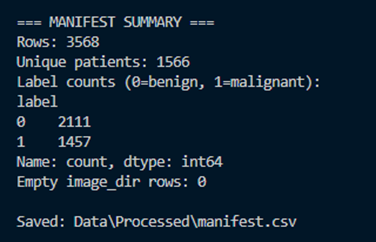
\includegraphics[width=0.95\linewidth]{figures/featureprototype/terminal1.png}
  \caption{Terminal output from the preprocessing/manifest step.}
  \label{fig:terminal1}
\end{figure}

To prevent data leakage, the dataset is split at the patient level rather than the image level, something that I explored in the literature review and the design section of the report. This is a critical consideration in medical imaging tasks, where multiple images from the same patient can otherwise appear in both training and evaluation sets, leading to inflated performance estimates. The splitting logic is implemented in \texttt{split\_data.py} using scikit-learn’s GroupShuffleSplit, with the patient identifier used as the grouping variable. The data is divided into training, validation, and test subsets according to proportions defined in the configuration file, ensuring that no patient appears in more than one split.

\texttt{Split\_data.py}, how GroupShuffleSplit is used with \texttt{patient\_id} as the grouping variable:

\lstinputlisting[
  language=Python,
  firstline=6,
  lastline=47,
    caption={how GroupShuffleSplit is used with \texttt{patient\_id} as the grouping variable in \texttt{split\_data.py}},
    label={lst:split_data}
]{../SRC/split_data.py}

Image loading and preprocessing are handled by a custom PyTorch Dataset class implemented in dataset.py. Because CBIS-DDSM images are stored as DICOM files, standard image loading utilities wouldn’t be sufficient. Instead, I used the pydicom library to read pixel data directly from the DICOM files. For this baseline implementation, a single representative DICOM image is loaded from each image series directory. Pixel intensities are normalised to the range [0, 1] to stabilise training, and images are resized to a fixed resolution compatible with the CNN architecture. Other data augmentation, including random horizontal flips and small rotations, is applied during training to improve generalisation.

The architecture used in this project is ResNet, selected in line with the design decisions outlined in Chapter 3. Transfer learning is employed by initialising the network with ImageNet pretrained weights. Given that mammography images are grayscale, the first convolutional layer of the network is adapted to accept a single channel input by averaging the RGB weights. The final fully connected layer is replaced with a single output neuron, producing a single logit suitable for binary classification using a sigmoid based loss function.

Code snippet for \texttt{model.py}:

\lstinputlisting[
  language=Python,
  firstline=5,
  lastline=29,
    caption={Model definition and transfer learning setup in \texttt{model.py}},
    label={lst:model}
]{../SRC/model.py}

Training logic is implemented in \texttt{train.py}. This script loads the previously generated manifest, applies the patient-level splitting procedure, and constructs PyTorch data loaders for the training and validation sets. Model performance on the validation set is monitored at the end of each epoch, and the best performing model checkpoint is saved automatically. This ensures that evaluation is conducted on the most generalisable model rather than the final training state, which may be overfitted.

Training loop from \texttt{train.py}:

\lstinputlisting[
  language=Python,
  firstline=170,
  lastline=219,
    caption={Training loop in \texttt{train.py}},
    label={lst:train_loop}
]{../SRC/train.py}

The model was trained for 10 epochs using ResNet initialised with ImageNet pretrained weights. Validation performance was monitored at the end of each epoch, and the model checkpoint achieving the lowest validation loss was saved automatically.

Across training, both training loss and validation loss decreased steadily, indicating effective learning without immediate signs of severe overfitting. Validation accuracy improved from approximately 63\% after the first epoch to just over 70\% by the final epoch.

\begin{figure}[H]
  \centering
  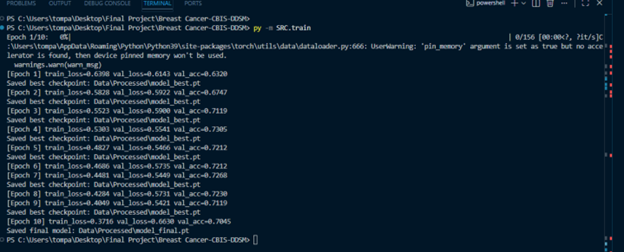
\includegraphics[width=0.95\linewidth]{figures/featureprototype/terminal2.png}
  \caption{Terminal output training over 10 epochs.}
  \label{fig:terminal2}
\end{figure}

Evaluation is performed using a separate script, eval.py, which loads the saved test split and the best model checkpoint. The model produces probability estimates for each test sample, which are then used to compute relevant evaluation metrics. These metrics include the area under the receiver operating characteristic curve (AUC), precision, recall (sensitivity), specificity, F1 score, and confusion matrix values. The results are printed to the terminal for inspection and saved to a structured JSON file to support reproducibility and reporting. Whilst this is presentable, I am considering an implementation which better displays the result, possibly with some kind of GUI. However, this would be a late project extension if that was a direction in which I wished to take the project once fully operational.

Final evaluation was conducted on a held-out test set containing data from patients unseen during training and validation. The best performing model checkpoint was loaded and used to generate probabilistic predictions for each test sample. At a decision threshold of 0.5, the model achieved the following results:

\begin{figure}[H]
  \centering
    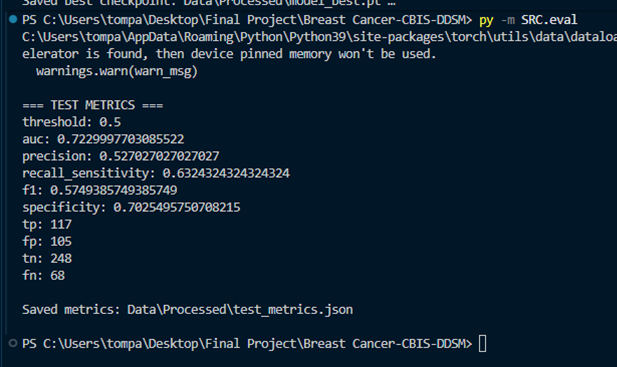
\includegraphics[width=0.95\linewidth]{figures/featureprototype/terminal3.png}
    \caption{Terminal output from the evaluation step.}
    \label{fig:terminal3}
\end{figure}

The confusion matrix at this threshold contained 117 true positives, 248 true negatives, 105 false positives, and 68 false negatives. These results indicate that the model demonstrates reasonable discriminative ability, with particular strength in sensitivity relative to random or majority class baselines.

While false positives remain relatively high, this does give a solid foundation to build upon as the project moves forward.

The prototype demonstrates that the proposed system design is technically feasible and can be implemented in a structured, reproducible manner. The modular architecture allows individual components to be modified or extended independently, such as replacing the backbone network, incorporating class weighting to address imbalance, or extending the dataset loader to use multiple DICOM images per study.